\chapter{Análise dos dados obtidos}
\label{cap7}

\section{Resultados obtidos}

Tendo em vista os gráficos gerados por meio das bibliotecas \textit{MatplotLib, Wordcloud} \cite{gfg3} \cite{va1} e também os do \textit{software PowerBI}  foi possível reunir um grande conjunto de informação para realizar uma análise dos melhores pontos turísticos que todos os estabelecimentos locais, como hotéis, restaurantes e atracções, para além do património histórico-cultural podem oferecer e assim melhorar possíveis pontos negativos e positivos, ou então prever quais as atracções/hotéis/restaurantes que mais cativam os turistas.

Assim sendo, foram gerados gráficos para cada hotel/restaurante/atracção dos \textit{websites Tripadvisor, Booking e Zomato} usando as bibliotecas mencionadas com o intuito dos resultados serem mais facilmente visíveis com as \textit{keywords} mais usadas para mencionar cada um dos pontos turísticos, assim como um mapa da cidade de Beja que contém todas as \textit{keywords} e as percentagens entre sentimentos positivos e negativos.

Por fim foram gerados também gráficos com as informações ao longo do tempo dos mesmos \textit{websites} referidos, acerca dos sentimentos de cada ponto turístico utilizando o \textit{software PowerBI}.

\subsection{Resultados de totais}

\begin{figure}[!htb]
\centering
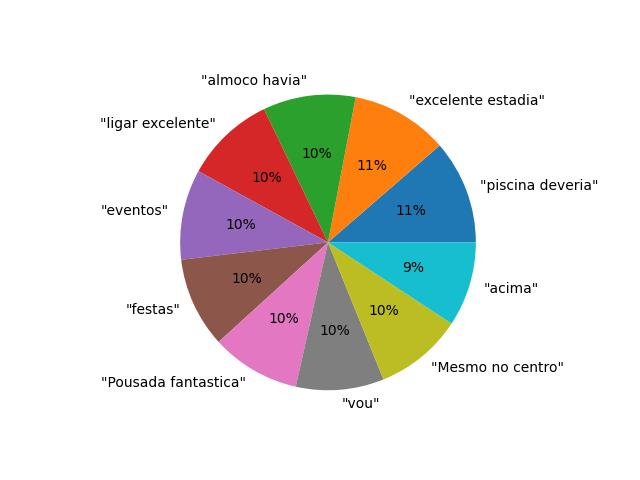
\includegraphics[width=14cm]{figuras/TripAdvisor/Hotels/hotel0_keywords.jpeg}
\caption{Gráfico circular com as \textit{keywords} mais usadas para a Pousada Convento Beja}
\label{fig:top10keywpcbeja}
\end{figure}

\begin{figure}[!htb]
\centering
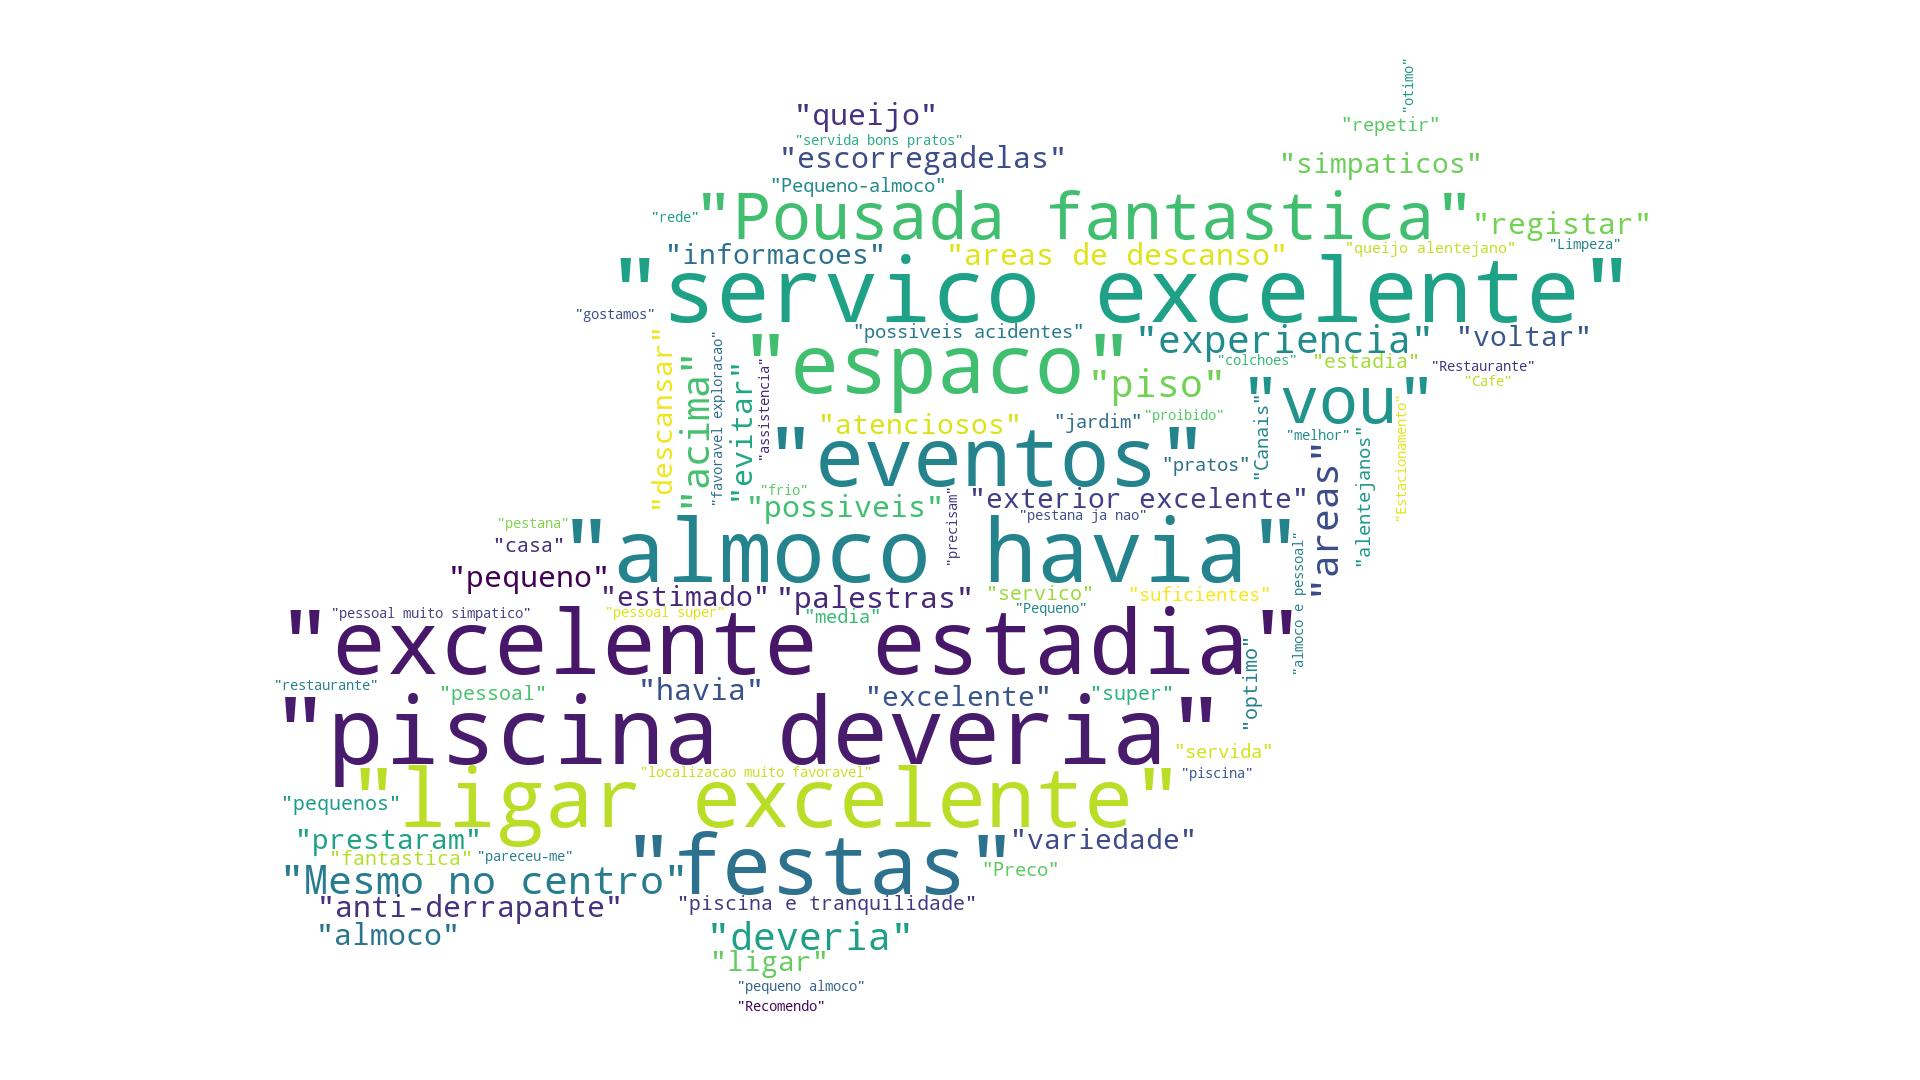
\includegraphics[width=14cm]{figuras/TripAdvisor/Hotels/hotel0_keywordcloud.jpeg}
\caption{Mapa de Beja com as \textit{keywords} mais usadas para a Pousada Convento Beja no seu interior}
\label{fig:top100keywcpcbeja}
\end{figure}

\begin{figure}[!htb]
\centering
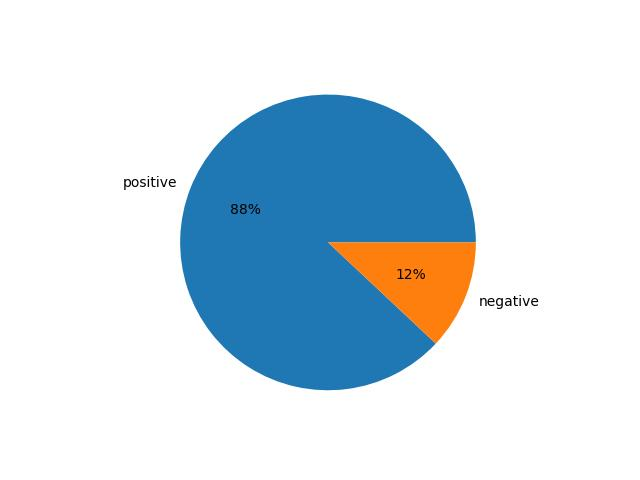
\includegraphics[width=14cm]{figuras/TripAdvisor/Hotels/hotel0_sentiments.jpeg}
\caption{Gráfico circular a representar a diferença entre os sentimentos positivos e negativos na Pousada Convento Beja}
\label{fig:sentpercetpcbeja}
\end{figure}

Nas figuras apresentadas acima são mostrados alguns resultados gerados pelas bibliotecas mencionadas, dos quais podemos notar que existe uma maioria para a quantidade de sentimentos positivos em relação aos negativos e que a maior parte das \textit{keywords} são também positivas. Porém, estes valores são retirados no momento em que a extracção dos dados foi realizada e não é possível verificar à medida do tempo como esses valores foram surgindo. Os valores entre restaurantes/hotéis/atracções é bastante semelhante entre si e então foi decidido que só iria ser mostrado alguns exemplos da realização desta etapa e todos os resultados ficariam mostrados nos anexos.

\subsection{Resultados temporais}

\begin{figure}[!htb]
\centering
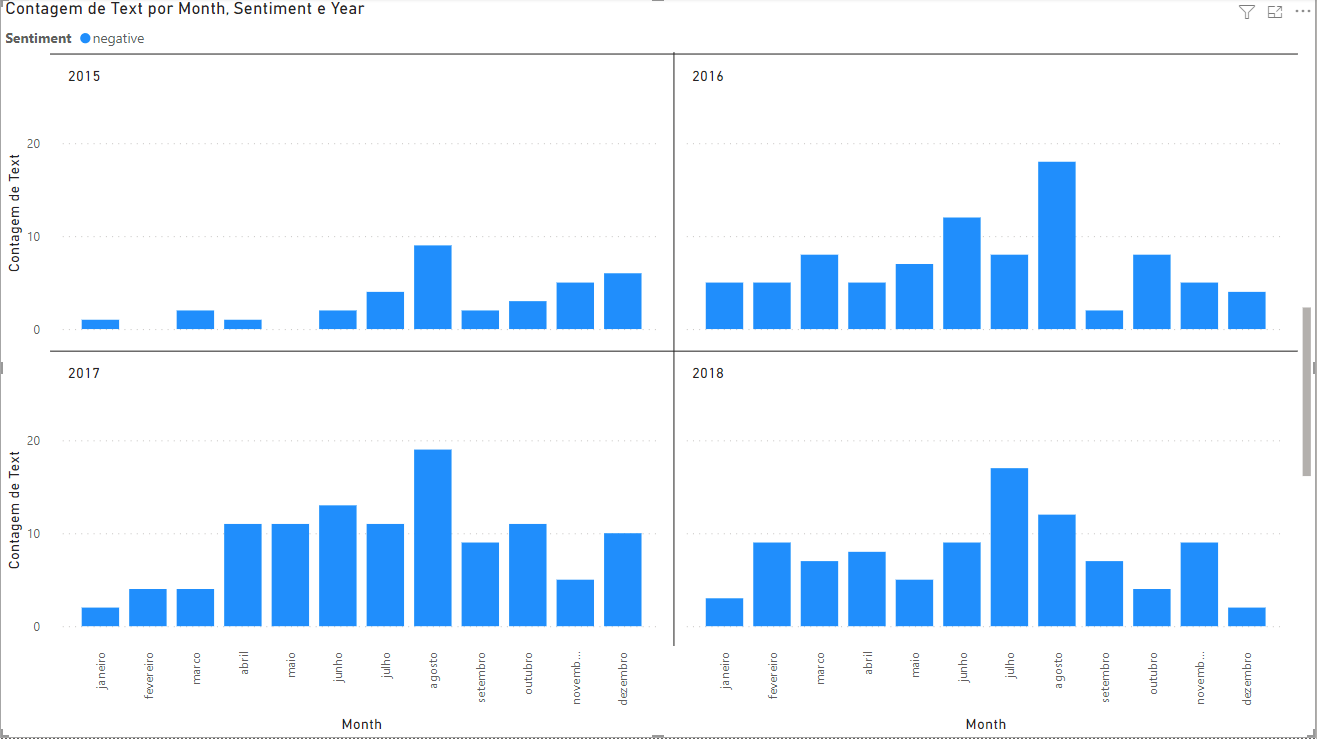
\includegraphics[width=16cm]{figuras/NegPerYear/1.PNG}
\caption{Gráfico de tabelas com a quantidade de sentimentos negativos ao longo do ano de cada hótel}
\label{fig:sentpercentbejatimed}
\end{figure}

\begin{figure}[!htb]
\centering
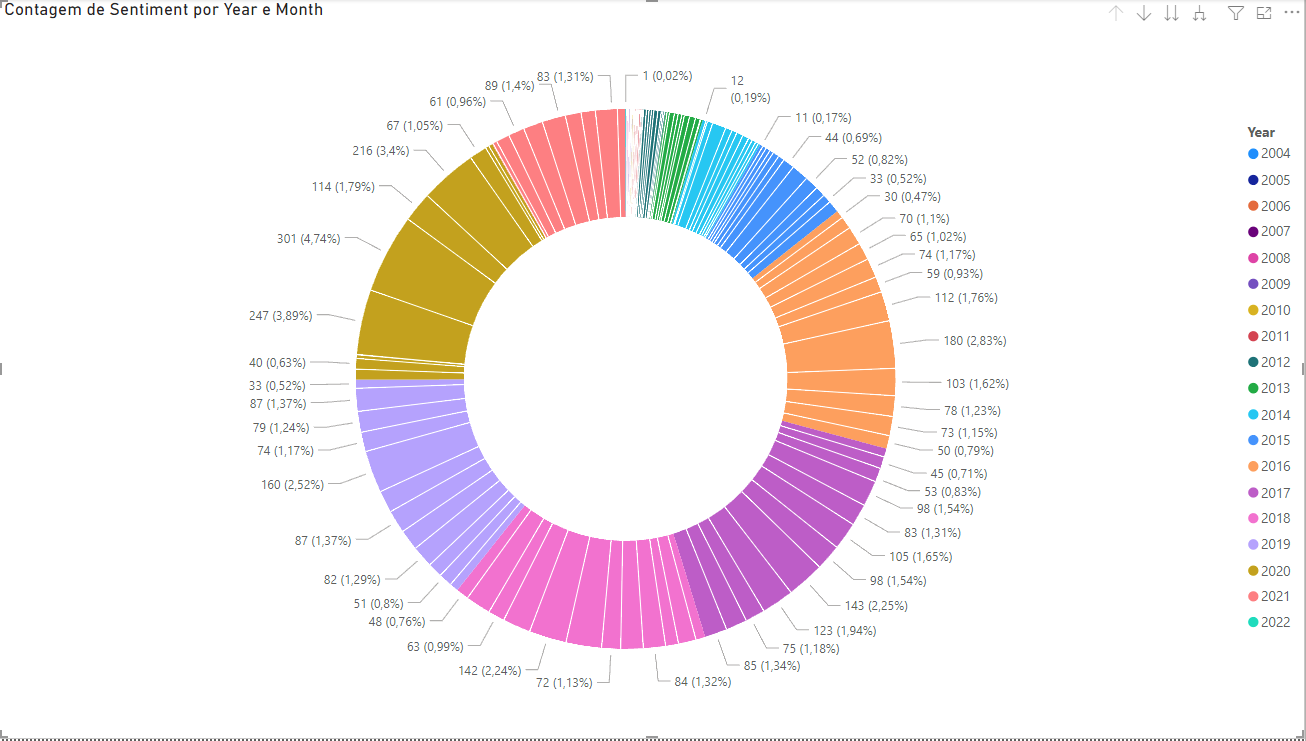
\includegraphics[width=16cm]{figuras/NrReviewsPerYear/CircleGraph.PNG}
\caption{Gráfico circular com a quantidade de \textit{reviews} ao longo do ano}
\label{fig:revspercentbejatimed}
\end{figure}

\begin{figure}[!htb]
\centering
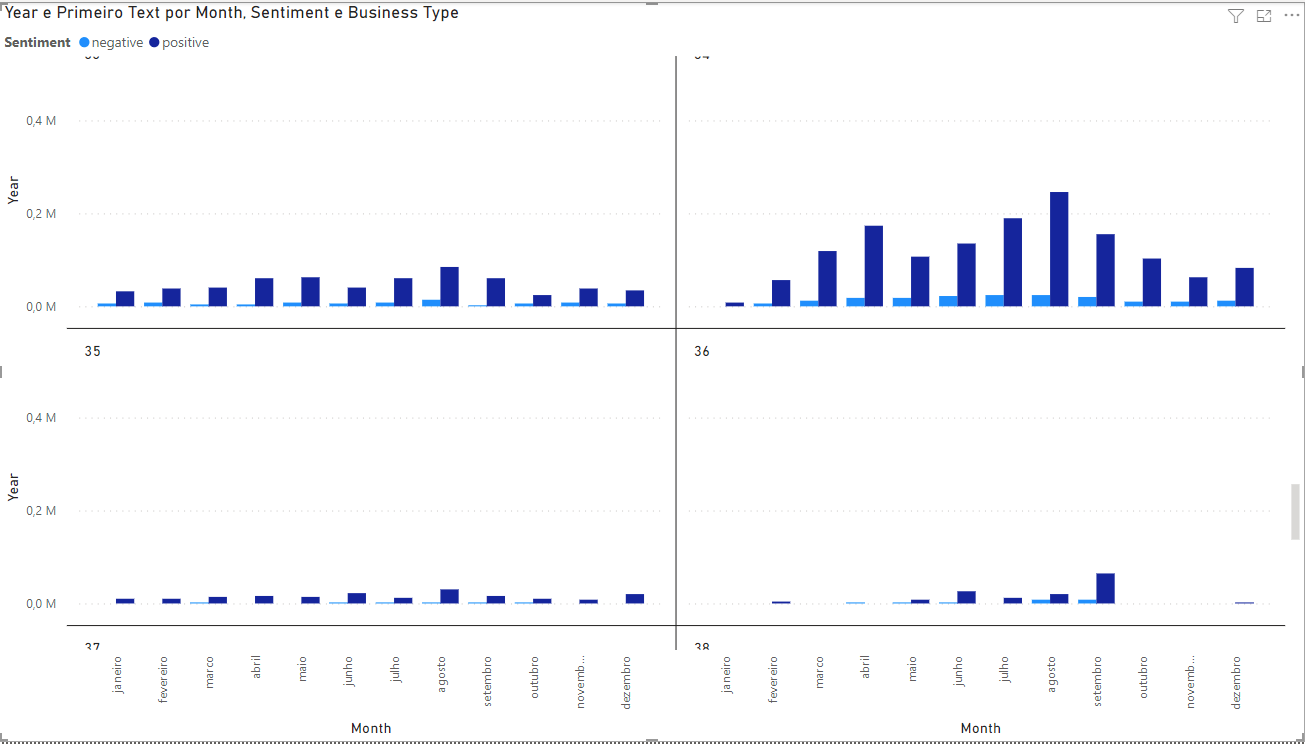
\includegraphics[width=16cm]{figuras/Pos&NegSentimentsPerMonth&BusinessType/2.PNG}
\caption{Gráfico de tabelas com a quantidade de sentimentos ao longo do ano por cada estabelecimento}
\label{fig:sentvarbejatimed}
\end{figure}

As figuras apresentadas desta vez foram elaboradas com o valor temporal bastante visível, sendo possível verificar desta vez uma evolução com o decorrer do tempo dos valores apresentados, assim como a forte diferença entre a quantidade de sentimentos escritos em meses onde um grande número de pessoas adere aos serviços, como no verão, Páscoa ou Natal.

\section {Análise dos resultados}

Graças a estes gráficos podemos concluir que as opiniões acerca do turismo cultural na zona alentejana é bastante positiva, mostrando uma enorme maioria de comentários positivos contra uma pequena quantidade de comentários negativos \hyperref[fig:sentvarbejatimed]{\textbf{como mostra esta figura}}. Podemos também notar que existem muitas mais pessoas a dar as suas opiniões em meses como Junho, Julho e Agosto, muito possivelmente devido á abertura das épocas balneares que movem grandes grupos de turistas nacionais e estrangeiros a fazerem férias pelas zonas costeiras que o Alentejo consegue fornecer com enorme facilidade graças ás magnificas praias na sua zona costeira. Por fim também é possível notar a evolução no número de opiniões com o decorrer dos anos e com a popularidade que o \textit{website} vai conseguindo, já que no começo o número de opiniões é baixo, porém com o passar dos anos começa a subir em elevado número.

É interessante também realçar um detalhe acerca de um gráfico em específico que o grupo decidiu não passar em branco. Olhemos para o seguinte gráfico.

\begin{figure}[!htb]
\centering
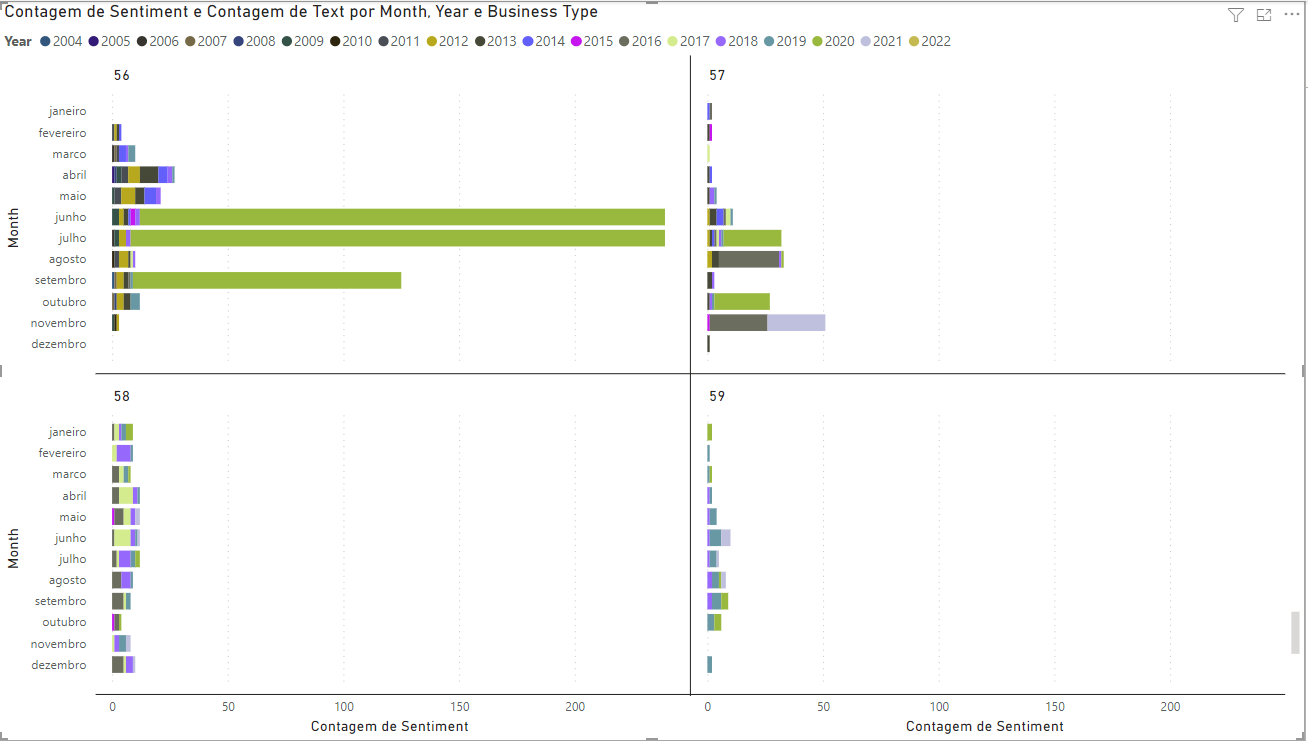
\includegraphics[width=16cm]{figuras/NrReviewsPerYear&BusinessType/9.PNG}
\caption{Gráfico de tabelas com a quantidade de sentimentos ao longo do ano por cada estabelecimento com valores diferentes}
\label{fig:figStrange}
\end{figure}

O Palácio dos Maldonados contém valores interessantes nos meses de Junho e Julho. São interessantes uma vez que durante o ano de 2020 o país se encontrava em confinamento devido á COVID-19, não sendo possível que ajuntamentos fossem realizados, porém foi verificado através do gráfico que o mesmo não se parece verificar já que existe uma brutal subida no número de pessoas a dar a sua opinião acerca da estadia que realizou, o que dá a entender que esse estabelecimento continuou a realizar as suas tarefas com normalidade ao contrário de outros que provavelmente seguiram as normas recomendadas.